\documentclass[12pt,letterpaper]{article}
\usepackage{inverba}
\newcommand{\userName}{Cullyn Newman}
\newcommand{\class}{BI 336} 
\newcommand{\institution}{Portland State University} 
\newcommand{\thetitle}{\hypertarget{home}{Cellular Biology}}
\rfoot{\hyperlink{home}{10 --- \thepage}}

\begin{document}
%%%%%%%%%%%%%%%%%%%%%%%%%%%%%%%%%%%%%%%%%%%%%%%%%%%%%%%%%%%%%%%%%%%%%%%%%%%%%%%%%%%%%%%%%
%                               %   %   %   %   %   %   %                               %
%                           %   %   %   %   %   %   %   %   %                           %
%                       %   %                               %   %                       %
%   %   %   %   %   %   %   %   O   U   T   L   I   N   E   %   %   %   %   %   %   %   %
%                       %   %                               %   %                       %
%                           %   %   %   %   %   %   %   %   %                           %
%                               %   %   %   %   %   %   %                               %
%%%%%%%%%%%%%%%%%%%%%%%%%%%%%%%%%%%%%%%%%%%%%%%%%%%%%%%%%%%%%%%%%%%%%%%%%%%%%%%%%%%%%%%%%

\begin{chapbox}{Cellular Biology}{ 
\begin{enumerate}[font=\bfseries, wide]
    \setcounter{enumi}{9}
    \item \hyperlink{10}{\textbf{Membrane Structure}}
    \begin{itemize}
        \item \hyperlink{10.1}{The Lipid Bilayer}
        \item \hyperlink{10.2}{Membrane Proteins}
    \end{itemize}
    \item \hyperlink{11}{\textbf{Transport Across Membrane}}
    \begin{itemize}
        \item
    \end{itemize}
    \item \hyperlink{12}{\textbf{Intracellular Transport}}
    \begin{itemize}
        \item 
    \end{itemize}
    \item \hyperlink{13}{\textbf{Vesicular Trafficking, Secretion, \& Endocytosis}}
    \begin{itemize}
        \item
    \end{itemize}
    \item \hyperlink{14}{\textbf{Energy Conversion: Mitochondria and Chloroplasts}}
    \begin{itemize}
        \item 
    \end{itemize}
    \item \hyperlink{15}{\textbf{Cellular Communication}}
    \begin{itemize}
        \item 
    \end{itemize}
    \item \hyperlink{16}{\textbf{The Cytoskeleton}}
    \begin{itemize}
        \item 
    \end{itemize}
    \item \hyperlink{17}{\textbf{The Cell Cycle}}
    \begin{itemize}
        \item 
    \end{itemize}
    \item \hyperlink{18}{\textbf{Apoptosis}}
    \begin{itemize}
        \item 
    \end{itemize}
    \item \hyperlink{19}{\textbf{Cell Interactions}}
    \begin{itemize}
        \item 
    \end{itemize}
    \item \hyperlink{20}{\textbf{Cancer}}
    \begin{itemize}
        \item 
    \end{itemize}    
    \item[22.] \hyperlink{22}{\textbf{Stem Cells and Tissue Renewal}}
    \begin{itemize}
        \item 
    \end{itemize}
    \item[24.] \hyperlink{24}{\textbf{The Innate and Adaptive Immune System}}
    \begin{itemize}
        \item 
    \end{itemize}
\end{enumerate}
}\end{chapbox}

%%%%%%%%%%%%%%%%%%%%%%%%%%%%%%%%%%%%%%%%%%%%%%%%%%%%%%%%%%%%%%%%%%%%%%%%%%%%%%%%%%%%%%%%%
%                               %   %   %   %   %   %   %                               %
%                           %   %   %   %   %   %   %   %   %                           %
%                       %   %                               %   %                       %
%   %   %   %   %   %   %   %       N   O   T   E   S       %   %   %   %   %   %   %   %
%                       %   %                               %   %                       %
%                           %   %   %   %   %   %   %   %   %                           %
%                               %   %   %   %   %   %   %                               %
%%%%%%%%%%%%%%%%%%%%%%%%%%%%%%%%%%%%%%%%%%%%%%%%%%%%%%%%%%%%%%%%%%%%%%%%%%%%%%%%%%%%%%%%%

%%%%%%%%%%%%%%%%%%%%%%%%%%%%%%%%%%%%%%%%%%%%%%%%%%%%%%%%%%%%%%%%%%%%%%%%%%%%%%%%%%%%%%%%%
\clearpage

\renewcommand{\thetitle}{\hypertarget{10}{The Genetic Code of Genes
and Genomes}}
\rfoot{\hyperlink{10}{10 --- \thepage}}
\hypertarget{10}{} 

%%%%%%%%%%%%%%%%%%%%%%%%%%%%%%%%%%%%%%%%%%%%%%%%%%%%%%%%%%%%%%%%%%%%%%%%%%%%%%%%%%%%%%%%%

\begin{chapbox}{\hyperlink{home}{Chapter 10: The Cell Membrane}}
    \begin{enumerate}
        \item \hyperlink{10.1}{The Lipid Bilayer}
        \item \hyperlink{10.2}{Membrane Proteins}
    \end{enumerate}
\end{chapbox}

%%%%%%%%%%%%%%%%%%%%%%%%%%%%%%%%%%%%%%%%%%%%%%%%%%%%%%%%%%%%%%%%%%%%%%%%%%%%%%%%%%%%%%%%%%
%  vvvvvvvvvvvvvvvvvvvvvvvvvvvvvvvvv   Section 10.1   vvvvvvvvvvvvvvvvvvvvvvvvvvvvvvvvv  %
\hypertarget{10.1}{}
\begin{secbox}{\hyperlink{10}{The Lipid Bilayer}}{
    \subsection*{Phosphoglycerides, Sphingolipids, and Sterols Are the Major
    Lipids in Cell Membranes}
    \begin{itemize}
        \item \textbf{Plasma membrane}: the part of the cell that separates the exterior and the interior of a cell with a semipermeable lipid bilayer. The plasma membrane regulates import and export of materials for the cell and includes various proteins that interact with other cells. 
        \item \textbf{Lipid bilayer}: the resulting structure of the spontaneous alignment of mostly amphiphilic phospholipids. 
        \item \textbf{Amphiphilic}: a chemical compound possessing a polar \textbf{hydrophilic} component and a \textbf{hydrophobic}, or lipophilic (fat loving), non polar end.
        \item \textbf{Phospholipids}: the most abundant membrane lipid containing a polar head consisting of a phosphate group and two hydrophobic fatty acid tails made of hydrocarbons.
        \item \textbf{Phosphoglycerides}: the main compounds that make up the phospholipids in animal cells, consisting of have a three-carbon glycerol backbone. Different combinations of head groups and tails can yield different phosphoglycerides. The most notable are: phosphatidylethanolamine, phosphatidylserine, and phosphatidylcholine.
        \item \textit{Sphingolipids}: similar to phosphoglycerides, but made up of sphingosine rather than glycerol.
        \item \textbf{Cholesterol}: a \textit{sterol} containing a rigid ring structure and attached to a single polar hydroxyl group. Cholesterol sits in the middle of the bilayer and helps provide structure by reducing tail mobility. 
    \end{itemize}

    \subsection*{The Lipid Bilayer Is a Two-dimensional Fluid}
    \begin{itemize}   
        \item \textbf{Liposomes}: a spherical with at least one lipid bilayer, most often made up of phospholipids, especially phosphatidylcholine.
        \item \textit{Phospholipid translocators}, or flippases, move phospholipids from the exoplasmic face (outside), to the cytosolic face (inside) of a lipid bilayer. Floppases move phospholipids in the inverse direction. 
        \item Fluidity depends on both composition and temperature. 
        \item \textit{Cis}-double bonds form kinks in the hydrocarbon tails, which make it harder to the tails to fit uniformly and constant movement within the bilayer.
        \item The addition of cholesterol decrease fluidity, but at the same time, high concentrations found in most eukaryotic plasma membranes also prevents the hydrocarbon chains from coming together and crystallizing.\par
        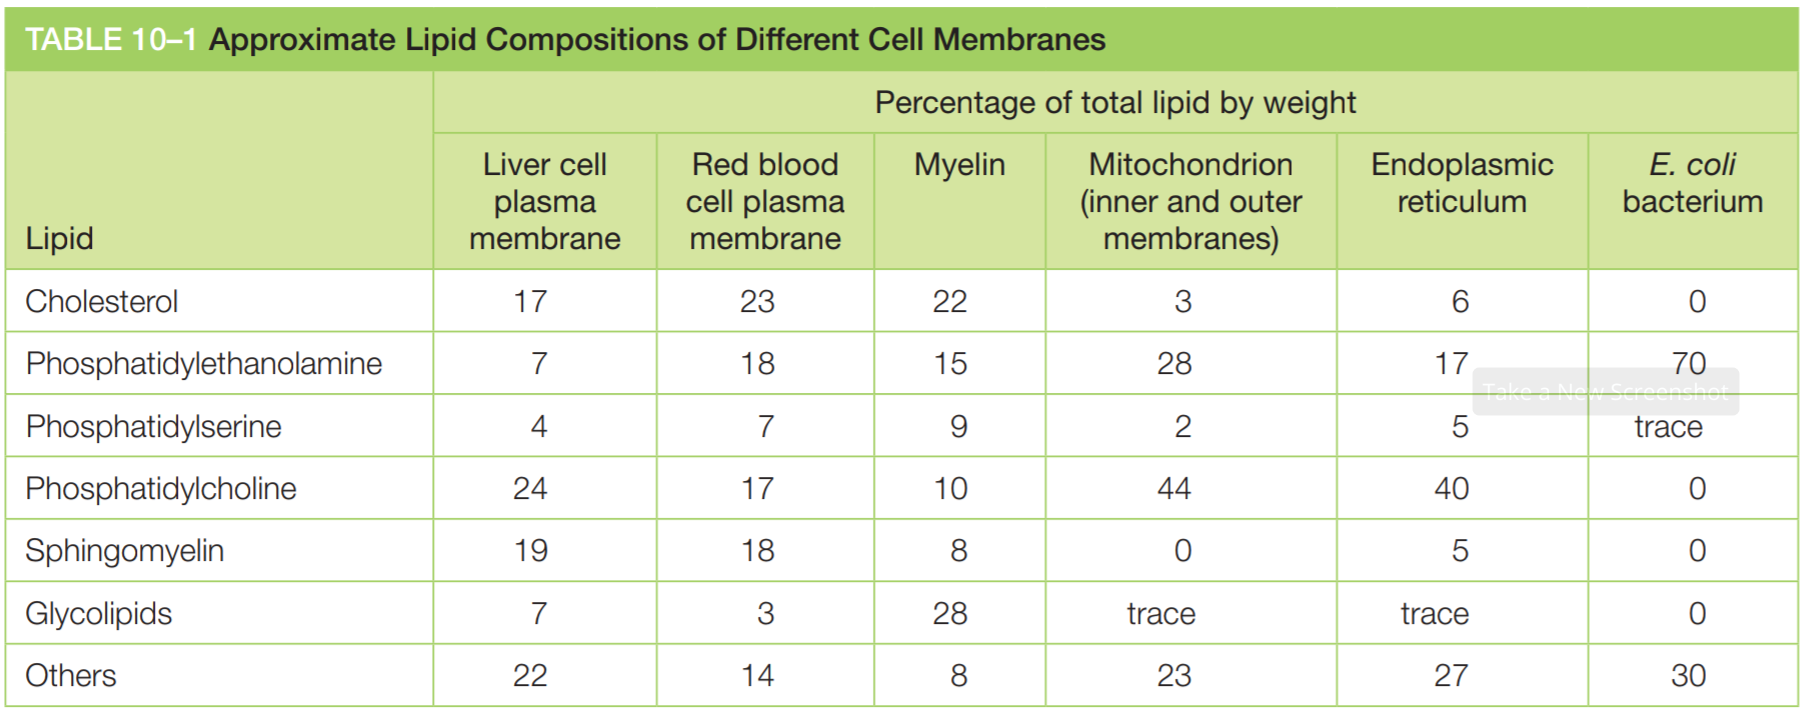
\includegraphics[width=\linewidth]{images/table_10_1.png}
    \end{itemize}

    \subsection*{Despite Their Fluidity, Lipid Bilayers Can Form Domains of Different Compositions}
    \begin{itemize}
        \item \textbf{Lipid raft}: specialized domains, or regions, that are enriched with particular lipids and cholesterol that allow for specialized associations with different cellular proteins. 
        \item Lipid rafts are dynamic structures, often coming together or splitting apart.\
        \item Lipid rafts influence membrane fluidity and membrane protein trafficking,
        \item Although more common in the cell membrane, lipid rafts have also been reported in other parts of the cell, such as the Golgi apparatus and lysosomes.
    \end{itemize}

    \subsection*{Lipid Droplets Are Surrounded by a Phospholipid Monolayer}
    \begin{itemize}
        \item \textbf{Lipid droplets}: lipid-rich cellular organelles that regulate the storage and hydrolysis of neutral lipids and are found largely in the adipose (fat) tissue. 
        \item Lipid droplets also serve as a reservoir for cholesterol and acyl-glycerols for membrane formation and maintenance.
        \item Generally, lipid droplets form rapidly in high concentration of fatty acids and generally form from discrete regions of the endoplasmic reticulum membrane where many enzymes of lipid metabolism are concentrated.
    \end{itemize}

    \subsection*{The Asymmetry of the Lipid Bilayer Is Functionally Important}
    \begin{itemize}
        \item The lipid compositions of the two monolayers of the lipid bilayer in many membranes are strikingly different.
        \item Lipid asymmetry is functionally important, especially in converting extracellular signals into intracellular ones, as many cytosolic proteins bind to specific lipid head groups found in the cytosolic monolayer of the lipid bilayer. 
        \item Animals exploit the phospholipid asymmetry of their plasma membranes to
        distinguish between live and dead cells. 
    \end{itemize}
    
    \subsection*{Glycolipids Are Found on the Surface of All Eukaryotic Plasma Membranes}
    \begin{itemize}
        \item \textbf{Glycolipids}: lipids with a carbohydrate attached by a glycosidic (covalent) bond.
        \item Glycolipids maintain the stability of the cell membrane and to facilitate cellular recognition, and are found on the surface of probably all eukaryotic cell membranes, where they extend from the phospholipid bilayer into the extracellular environment. 
        \item Glycolipids generally constitute about 5\% of the lipid molecules in the outer monolayer. 
        \item \textbf{Gangliosides}: a glycolipid that contain oligosaccharides (a polymer contain typically three to ten monosaccharides) with one or more sialic acid (an acidic sugar with a nine-carbon backbone), which produce a net negative charge.
        \item  Gangliosides are found predominantly in the nervous system where they constitute 6\% of all phospholipids.
    \end{itemize}

    \begin{probbox}{The Lipid Bilayer: Summary}
        Biological membranes consist of a continuous double layer of lipid molecules in which membrane proteins are embedded. This lipid bilayer is fluid, with individual lipid molecules able to diffuse rapidly within their own monolayer. The membrane lipid molecules are amphiphilic. When placed in water, they assemble spontaneously into bilayers, which form sealed compartments. Although cell membranes can contain hundreds of different lipid species, the plasma membrane in animal cells contains three major classes—phospholipids, cholesterol, and glycolipids. Because of their different backbone structure, phospholipids fall into two subclasses—phosphoglycerides and sphingolipids. The lipid compositions of the inner and outer monolayers are different, reflecting the different functions of the two faces of a cell membrane. Different mixtures of lipids are found in the membranes of cells of different types, as well as in the various membranes of a single eukaryotic cell. Inositol phospholipids are a minor class of phospholipids, which in the cytosolic leaflet of the plasma membrane lipid bilayer play an important part in cell signaling: in response to extracellular signals, specific lipid kinases phosphorylate the head groups of these lipids to form docking sites for cytosolic signaling proteins, whereas specific phospholipases cleave certain inositol phospholipids to generate small intracellular signaling molecules.
    \end{probbox}
}\end{secbox}
%  ^^^^^^^^^^^^^^^^^^^^^^^^^^^^^^^^^   Section 10.1   ^^^^^^^^^^^^^^^^^^^^^^^^^^^^^^^^  %  
%%%%%%%%%%%%%%%%%%%%%%%%%%%%%%%%%%%%%%%%%%%%%%%%%%%%%%%%%%%%%%%%%%%%%%%%%%%%%%%%%%%%%%%%%%
%  vvvvvvvvvvvvvvvvvvvvvvvvvvvvvvvvvv  Section 10.2   vvvvvvvvvvvvvvvvvvvvvvvvvvvvvvvv  % 
\hypertarget{10.2}{}
\begin{secbox}{\hyperlink{10}{Membrane Proteins}}{
    \subsection*{Membrane Proteins Can Be Associated with the Lipid Bilayer in Various Ways}
    \begin{itemize}
        \item \textbf{Transmembrane protein}
        \item \textbf{Glycosylphosphatidylinositol (GPI) anchor}
        \item \textbf{Membrane-associated proteins}
    \end{itemize}
    
    \subsection*{Lipid Anchors Control the Membrane Localization of Some Signaling Proteins}
    \begin{itemize}
        \item
    \end{itemize}
    
    \subsection*{In Most Transmembrane Proteins, the Polypeptide Chain Crosses the Lipid Bilayer in an \(\bm{\alpha}\)-Helical Conformation}
    \begin{itemize}
        \item \textbf{Single pass transmembrane proteins}
        \item \textbf{Multi-pass transmembrane proteins}
    \end{itemize}
    
    \subsection*{Transmembrane \bfg{\alpha} Helices Often Interact with One Another}
    \begin{itemize}
        \item 
    \end{itemize}

    \subsection*{Some \bfg{\beta} Barrels Form Large Channels}
    \begin{itemize}
        \item \textbf{Lumen}
    \end{itemize}

    \subsection*{Many Membrane Proteins Are Glycosylated}
    \begin{itemize}
        \item \textbf{Carbohydrate layer}
        \item \textbf{Lectins}
    \end{itemize}

    \subsection*{Membrane Proteins Can Be Solubilized and Purified in Detergents}
    \begin{itemize}
        \item \textbf{Detergents}
    \end{itemize}

    \subsection*{Bacteriorhodopsin Is a Light-driven Proton H\bfg{^+} Pump That
    Traverses the Lipid Bilayer as Seven \bfg{\alpha} Helices}
    \begin{itemize}
        \item \textbf{Bacteriorhodopsin}
    \end{itemize}

    \subsection*{Some \bfg{\beta} Barrels Form Large ChannelsThe Cortical Cytoskeleton Gives Membranes Mechanical Strength and Restricts Membrane Protein Diffusion}
    \begin{itemize}
        \item \textbf{Spectrin}
        \item \textbf{Cortex}
    \end{itemize}

    \subsection*{Membrane-bending Proteins Deform Bilayers}
    \begin{itemize}
        \item \textbf{Membrane bending proteins}
    \end{itemize}
}\end{secbox}
%  ^^^^^^^^^^^^^^^^^^^^^^^^^^^^^^^^^   Section 10.2   ^^^^^^^^^^^^^^^^^^^^^^^^^^^^^^^  %  
%%%%%%%%%%%%%%%%%%%%%%%%%%%%%%%%%%%%%%%%%%%%%%%%%%%%%%%%%%%%%%%%%%%%%%%%%%%%%%%%%%%%%%%%%%
\end{document}